\documentclass{article}
\usepackage[utf8]{inputenc}

\title{Assignment-5\\Pipes and shared memory}
\author{Subash Mylraj \\(CED18I051) }
\date{25 October 2020}

\usepackage{geometry}
 \geometry{
 a4paper,
 total={170mm,257mm},
 left=20mm,
 top=10mm,
 }

\usepackage{longtable}
\usepackage{graphicx}
\usepackage{listings}
\usepackage{xcolor}

\begin{document}

\maketitle

\lstset{
  language=c,
  aboveskip=3mm,
  belowskip=3mm,
  showstringspaces=false,
  columns=flexible,
  basicstyle={\small\ttfamily},
  numbers=none,
  numberstyle=\tiny\color{gray},
  keywordstyle=\color{blue},
  commentstyle=\color{dkgreen},
  stringstyle=\color{mauve},
  breaklines=true,
  breakatwhitespace=true,
  tabsize=3
}

\definecolor{dkgreen}{rgb}{0,0.6,0}
\definecolor{gray}{rgb}{0.5,0.5,0.5}
\definecolor{mauve}{rgb}{0.58,0,0.82}

\section*{Question 1: Parent sets up a string which is read by child, reversed there and read back the parent}
\bigskip
\bigskip

\par\noindent
\textbf{\Large Code: }
\smallskip
\par\noindent\rule{\textwidth}{0.4pt}
\lstinputlisting[language=c]{src/1.c}
\par\noindent\rule{\textwidth}{0.4pt}

\bigskip
\noindent
\textbf{\Large Output:}

\begin{figure}[h]
	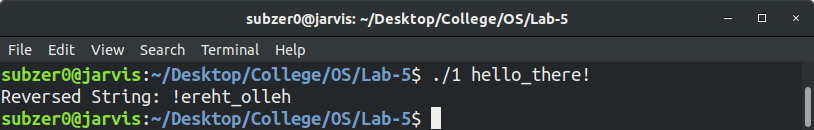
\includegraphics[width=\textwidth]{output/1.png}
\end{figure}
\bigskip

\section*{Question 2: Parent sets up string 1 and child sets up string 2. String 2 concatenated to string 1 at parent end and then read back at the child end.}
\bigskip
\bigskip

\par\noindent
\textbf{\Large Code: }
\smallskip
\par\noindent\rule{\textwidth}{0.4pt}
\lstinputlisting[language=c]{src/2.c}
\par\noindent\rule{\textwidth}{0.4pt}

\bigskip
\noindent
\textbf{\Large Output:}

\begin{figure}[h]
	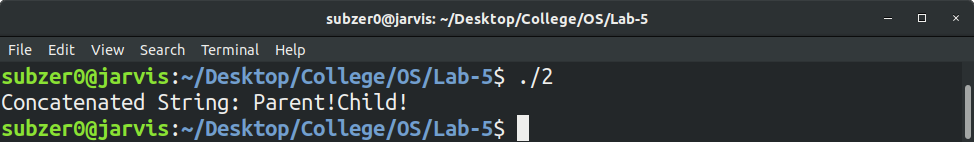
\includegraphics[width=\textwidth]{output/2.png}
\end{figure}
\bigskip

\section*{Question 3: Substring generation at child end of a string setup at parent process end.}
\bigskip
\bigskip

\par\noindent
\textbf{\Large Code: }
\smallskip
\par\noindent\rule{\textwidth}{0.4pt}
\lstinputlisting[language=c]{src/3.c}
\par\noindent\rule{\textwidth}{0.4pt}

\bigskip
\noindent
\textbf{\Large Explanation: } \\

Parent sends a string to child through a pipe. Child reads
the string and finds all the possible substrings and prints
it to terminal.
\pagebreak

\bigskip
\noindent
\textbf{\Large Output:}

\begin{figure}[h]
	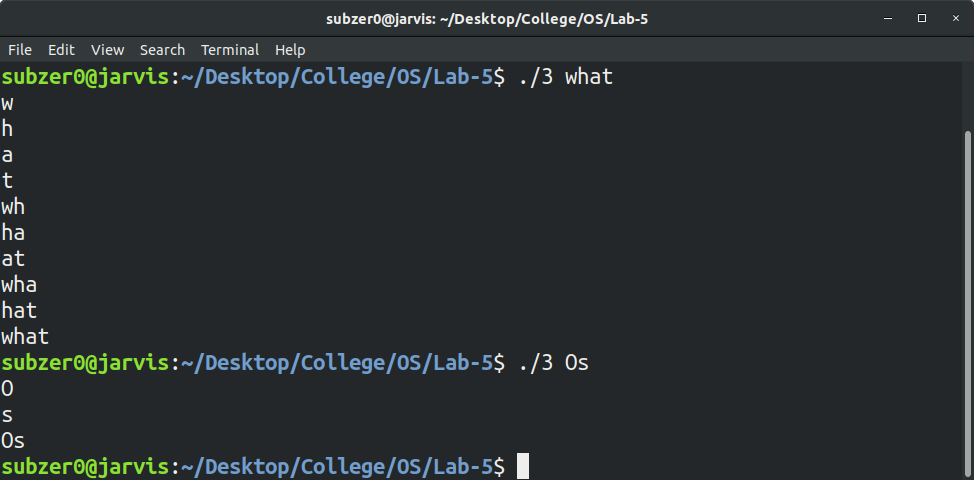
\includegraphics[width=\textwidth]{output/3.png}
\end{figure}
\bigskip

\section*{Question 4: String reversal and palindrome check using pipes / shared memory.}
\bigskip
\bigskip

\par\noindent
\textbf{\Large Code: }
\smallskip
\par\noindent\rule{\textwidth}{0.4pt}
\lstinputlisting[language=c]{src/4.c}
\par\noindent\rule{\textwidth}{0.4pt}

\bigskip
\noindent
\textbf{\Large Output:}

\begin{figure}[h]
	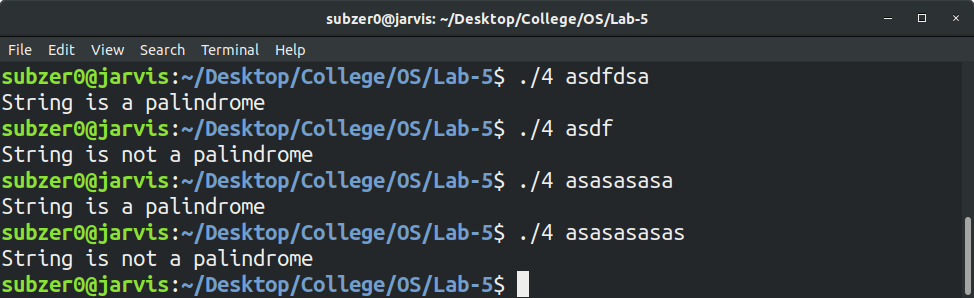
\includegraphics[width=\textwidth]{output/4.png}
\end{figure}
\bigskip


\section*{Question 5: Armstrong number generation within a range. The digit extraction, cubing can be responsibility of child while the checking for sum == no can happen in child and the output list in the child.}
\bigskip
\bigskip

\par\noindent
\textbf{\Large Code: }
\smallskip
\par\noindent\rule{\textwidth}{0.4pt}
\lstinputlisting[language=c]{src/5.c}
\par\noindent\rule{\textwidth}{0.4pt}

\bigskip
\noindent
\textbf{\Large Explanation: } \\


This program was done using shared memory. The parent forks
for every number in the range. The child processes find whether
the number they forked at is an armstrong number or not. If the
number is an armstrong number, then it is appended to an array
where all the armstrong numbers within that range are stored. This
array is made available to all the processes using shared memory. A 
structure was used to store both the array the next iterator to that
array.


\bigskip
\noindent
\textbf{\Large Output:}

\begin{figure}[h]
	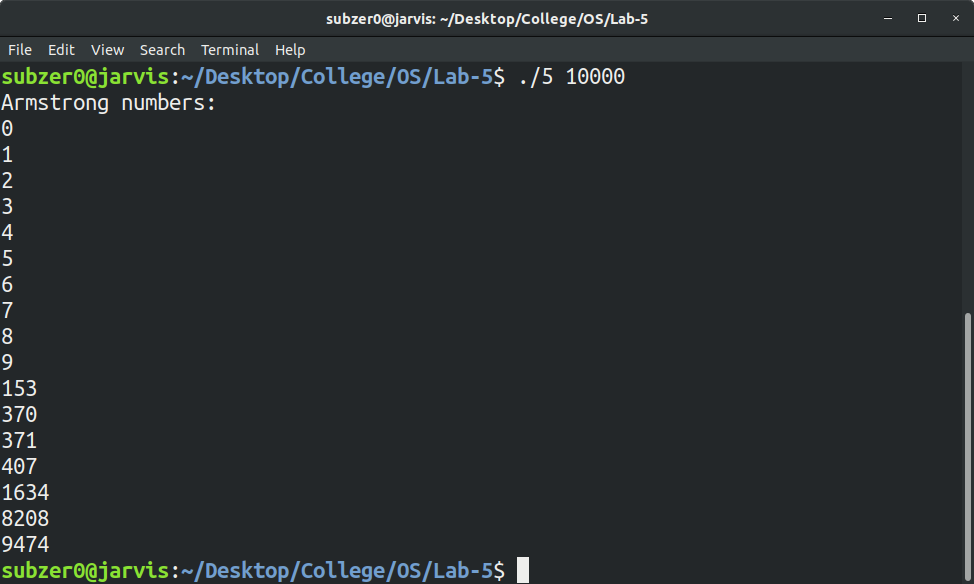
\includegraphics[width=\textwidth]{output/5.png}
\end{figure}
\bigskip

\end{document}